\documentclass[1p]{elsarticle_modified}
%\bibliographystyle{elsarticle-num}

%\usepackage[colorlinks]{hyperref}
%\usepackage{abbrmath_seonhwa} %\Abb, \Ascr, \Acal ,\Abf, \Afrak
\usepackage{amsfonts}
\usepackage{amssymb}
\usepackage{amsmath}
\usepackage{amsthm}
\usepackage{scalefnt}
\usepackage{amsbsy}
\usepackage{kotex}
\usepackage{caption}
\usepackage{subfig}
\usepackage{color}
\usepackage{graphicx}
\usepackage{xcolor} %% white, black, red, green, blue, cyan, magenta, yellow
\usepackage{float}
\usepackage{setspace}
\usepackage{hyperref}

\usepackage{tikz}
\usetikzlibrary{arrows}

\usepackage{multirow}
\usepackage{array} % fixed length table
\usepackage{hhline}

%%%%%%%%%%%%%%%%%%%%%
\makeatletter
\renewcommand*\env@matrix[1][\arraystretch]{%
	\edef\arraystretch{#1}%
	\hskip -\arraycolsep
	\let\@ifnextchar\new@ifnextchar
	\array{*\c@MaxMatrixCols c}}
\makeatother %https://tex.stackexchange.com/questions/14071/how-can-i-increase-the-line-spacing-in-a-matrix
%%%%%%%%%%%%%%%

\usepackage[normalem]{ulem}

\newcommand{\msout}[1]{\ifmmode\text{\sout{\ensuremath{#1}}}\else\sout{#1}\fi}
%SOURCE: \msout is \stkout macro in https://tex.stackexchange.com/questions/20609/strikeout-in-math-mode

\newcommand{\cancel}[1]{
	\ifmmode
	{\color{red}\msout{#1}}
	\else
	{\color{red}\sout{#1}}
	\fi
}

\newcommand{\add}[1]{
	{\color{blue}\uwave{#1}}
}

\newcommand{\replace}[2]{
	\ifmmode
	{\color{red}\msout{#1}}{\color{blue}\uwave{#2}}
	\else
	{\color{red}\sout{#1}}{\color{blue}\uwave{#2}}
	\fi
}

\newcommand{\Sol}{\mathcal{S}} %segment
\newcommand{\D}{D} %diagram
\newcommand{\A}{\mathcal{A}} %arc


%%%%%%%%%%%%%%%%%%%%%%%%%%%%%5 test

\def\sl{\operatorname{\textup{SL}}(2,\Cbb)}
\def\psl{\operatorname{\textup{PSL}}(2,\Cbb)}
\def\quan{\mkern 1mu \triangleright \mkern 1mu}

\theoremstyle{definition}
\newtheorem{thm}{Theorem}[section]
\newtheorem{prop}[thm]{Proposition}
\newtheorem{lem}[thm]{Lemma}
\newtheorem{ques}[thm]{Question}
\newtheorem{cor}[thm]{Corollary}
\newtheorem{defn}[thm]{Definition}
\newtheorem{exam}[thm]{Example}
\newtheorem{rmk}[thm]{Remark}
\newtheorem{alg}[thm]{Algorithm}

\newcommand{\I}{\sqrt{-1}}
\begin{document}

%\begin{frontmatter}
%
%\title{Boundary parabolic representations of knots up to 8 crossings}
%
%%% Group authors per affiliation:
%\author{Yunhi Cho} 
%\address{Department of Mathematics, University of Seoul, Seoul, Korea}
%\ead{yhcho@uos.ac.kr}
%
%
%\author{Seonhwa Kim} %\fnref{s_kim}}
%\address{Center for Geometry and Physics, Institute for Basic Science, Pohang, 37673, Korea}
%\ead{ryeona17@ibs.re.kr}
%
%\author{Hyuk Kim}
%\address{Department of Mathematical Sciences, Seoul National University, Seoul 08826, Korea}
%\ead{hyukkim@snu.ac.kr}
%
%\author{Seokbeom Yoon}
%\address{Department of Mathematical Sciences, Seoul National University, Seoul, 08826,  Korea}
%\ead{sbyoon15@snu.ac.kr}
%
%\begin{abstract}
%We find all boundary parabolic representation of knots up to 8 crossings.
%
%\end{abstract}
%\begin{keyword}
%    \MSC[2010] 57M25 
%\end{keyword}
%
%\end{frontmatter}

%\linenumbers
%\tableofcontents
%
\newcommand\colored[1]{\textcolor{white}{\rule[-0.35ex]{0.8em}{1.4ex}}\kern-0.8em\color{red} #1}%
%\newcommand\colored[1]{\textcolor{white}{ #1}\kern-2.17ex	\textcolor{white}{ #1}\kern-1.81ex	\textcolor{white}{ #1}\kern-2.15ex\color{red}#1	}

{\Large $\underline{12n_{0666}~(K12n_{0666})}$}

\setlength{\tabcolsep}{10pt}
\renewcommand{\arraystretch}{1.6}
\vspace{1cm}\begin{tabular}{m{100pt}>{\centering\arraybackslash}m{274pt}}
\multirow{5}{120pt}{
	\centering
	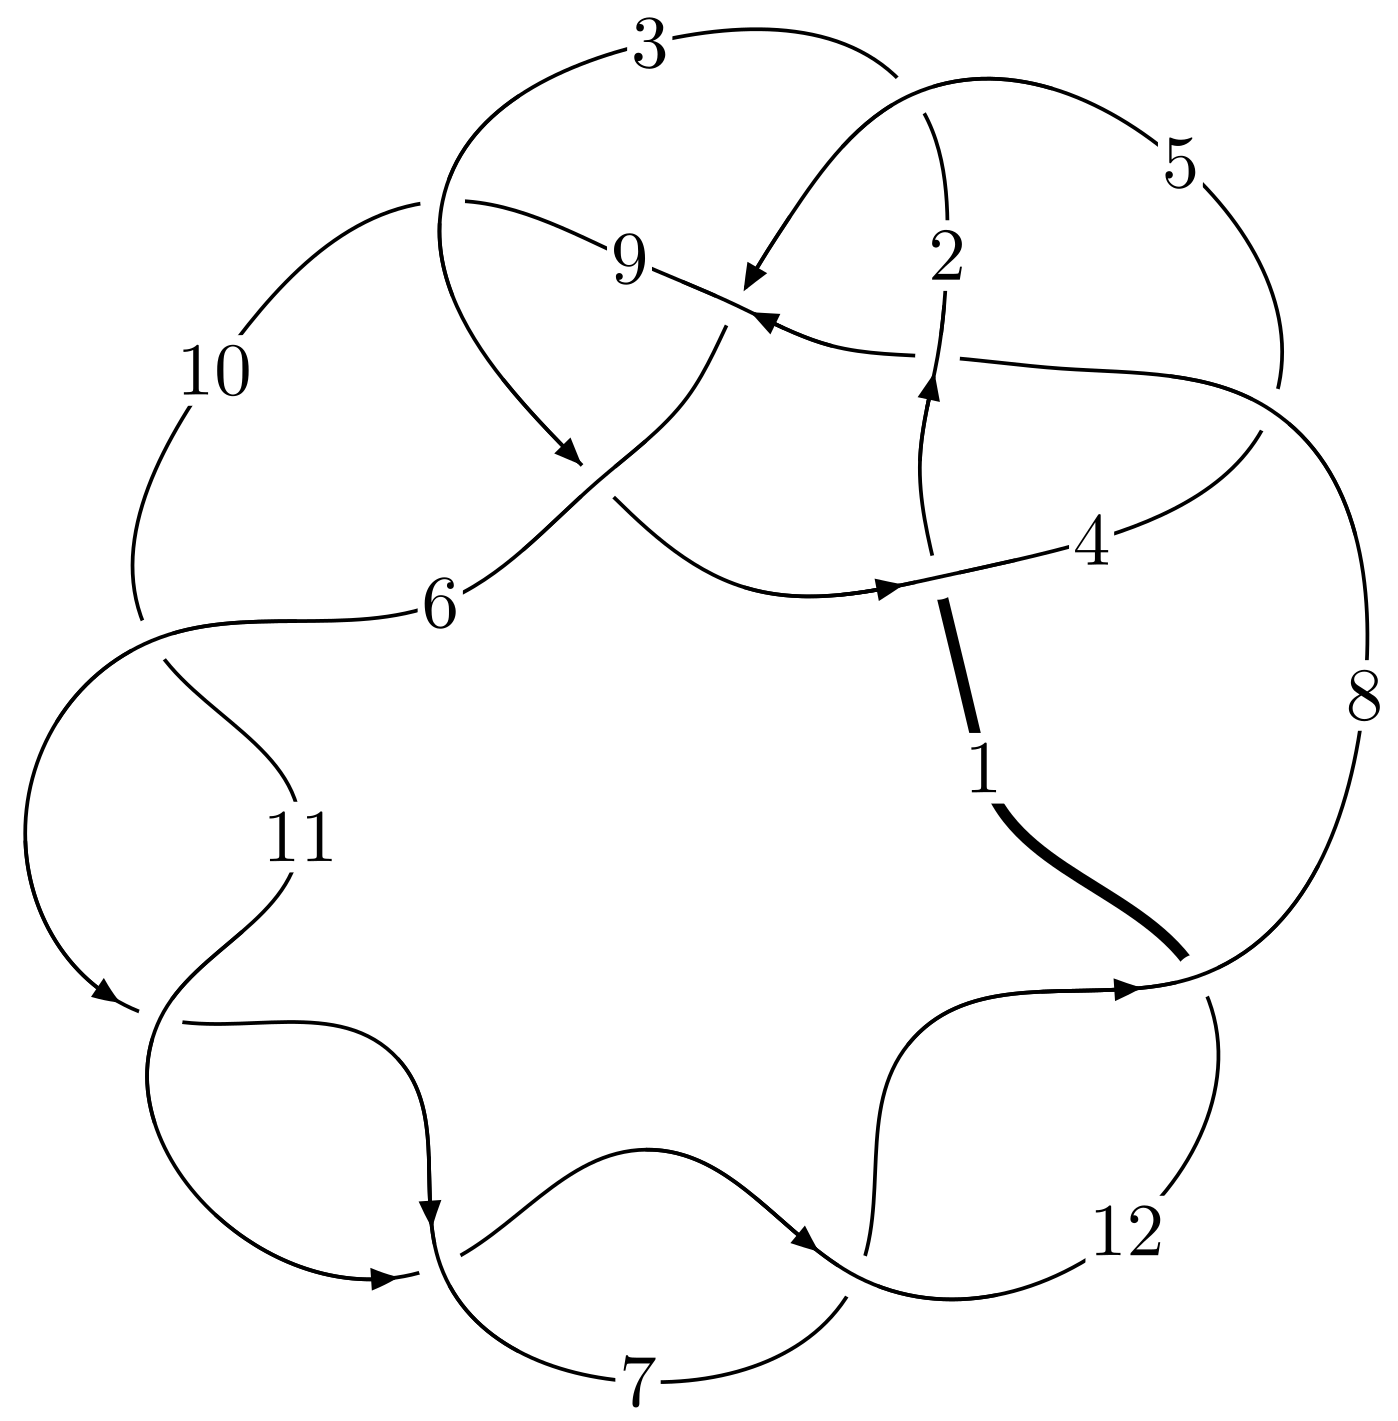
\includegraphics[width=112pt]{../../../GIT/diagram.site/Diagrams/png/2755_12n_0666.png}\\
\ \ \ A knot diagram\footnotemark}&
\allowdisplaybreaks
\textbf{Linearized knot diagam} \\
\cline{2-2}
 &
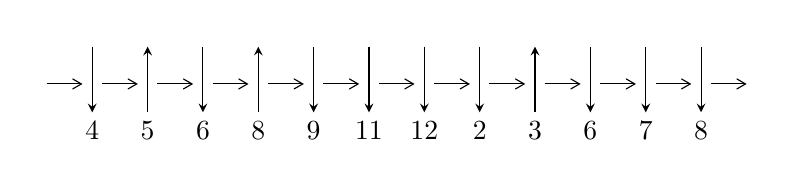
\begin{tikzpicture}[x=20pt, y=17pt]
	% nodes
	\node (C0) at (0, 0) {};
	\node (C1) at (1, 0) {};
	\node (C1U) at (1, +1) {};
	\node (C1D) at (1, -1) {4};

	\node (C2) at (2, 0) {};
	\node (C2U) at (2, +1) {};
	\node (C2D) at (2, -1) {5};

	\node (C3) at (3, 0) {};
	\node (C3U) at (3, +1) {};
	\node (C3D) at (3, -1) {6};

	\node (C4) at (4, 0) {};
	\node (C4U) at (4, +1) {};
	\node (C4D) at (4, -1) {8};

	\node (C5) at (5, 0) {};
	\node (C5U) at (5, +1) {};
	\node (C5D) at (5, -1) {9};

	\node (C6) at (6, 0) {};
	\node (C6U) at (6, +1) {};
	\node (C6D) at (6, -1) {11};

	\node (C7) at (7, 0) {};
	\node (C7U) at (7, +1) {};
	\node (C7D) at (7, -1) {12};

	\node (C8) at (8, 0) {};
	\node (C8U) at (8, +1) {};
	\node (C8D) at (8, -1) {2};

	\node (C9) at (9, 0) {};
	\node (C9U) at (9, +1) {};
	\node (C9D) at (9, -1) {3};

	\node (C10) at (10, 0) {};
	\node (C10U) at (10, +1) {};
	\node (C10D) at (10, -1) {6};

	\node (C11) at (11, 0) {};
	\node (C11U) at (11, +1) {};
	\node (C11D) at (11, -1) {7};

	\node (C12) at (12, 0) {};
	\node (C12U) at (12, +1) {};
	\node (C12D) at (12, -1) {8};
	\node (C13) at (13, 0) {};

	% arrows
	\draw[->,>={angle 60}]
	(C0) edge (C1) (C1) edge (C2) (C2) edge (C3) (C3) edge (C4) (C4) edge (C5) (C5) edge (C6) (C6) edge (C7) (C7) edge (C8) (C8) edge (C9) (C9) edge (C10) (C10) edge (C11) (C11) edge (C12) (C12) edge (C13) ;	\draw[->,>=stealth]
	(C1U) edge (C1D) (C2D) edge (C2U) (C3U) edge (C3D) (C4D) edge (C4U) (C5U) edge (C5D) (C6U) edge (C6D) (C7U) edge (C7D) (C8U) edge (C8D) (C9D) edge (C9U) (C10U) edge (C10D) (C11U) edge (C11D) (C12U) edge (C12D) ;
	\end{tikzpicture} \\
\hhline{~~} \\& 
\textbf{Solving Sequence} \\ \cline{2-2} 
 &
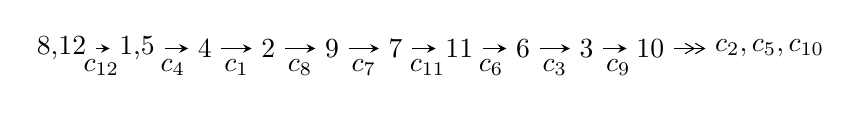
\begin{tikzpicture}[x=23pt, y=7pt]
	% node
	\node (A0) at (-1/8, 0) {8,12};
	\node (A1) at (17/16, 0) {1,5};
	\node (A2) at (17/8, 0) {4};
	\node (A3) at (25/8, 0) {2};
	\node (A4) at (33/8, 0) {9};
	\node (A5) at (41/8, 0) {7};
	\node (A6) at (49/8, 0) {11};
	\node (A7) at (57/8, 0) {6};
	\node (A8) at (65/8, 0) {3};
	\node (A9) at (73/8, 0) {10};
	\node (C1) at (1/2, -1) {$c_{12}$};
	\node (C2) at (13/8, -1) {$c_{4}$};
	\node (C3) at (21/8, -1) {$c_{1}$};
	\node (C4) at (29/8, -1) {$c_{8}$};
	\node (C5) at (37/8, -1) {$c_{7}$};
	\node (C6) at (45/8, -1) {$c_{11}$};
	\node (C7) at (53/8, -1) {$c_{6}$};
	\node (C8) at (61/8, -1) {$c_{3}$};
	\node (C9) at (69/8, -1) {$c_{9}$};
	\node (A10) at (11, 0) {$c_{2},c_{5},c_{10}$};

	% edge
	\draw[->,>=stealth]	
	(A0) edge (A1) (A1) edge (A2) (A2) edge (A3) (A3) edge (A4) (A4) edge (A5) (A5) edge (A6) (A6) edge (A7) (A7) edge (A8) (A8) edge (A9) ;
	\draw[->>,>={angle 60}]	
	(A9) edge (A10);
\end{tikzpicture} \\ 

\end{tabular} \\

\footnotetext{
The image of knot diagram is generated by the software ``\textbf{Draw programme}" developed by Andrew Bartholomew(\url{http://www.layer8.co.uk/maths/draw/index.htm\#Running-draw}), where we modified some parts for our purpose(\url{https://github.com/CATsTAILs/LinksPainter}).
}\phantom \\ \newline 
\centering \textbf{Ideals for irreducible components\footnotemark of $X_{\text{par}}$} 
 
\begin{align*}
I^u_{1}&=\langle 
- u^{15}+6 u^{13}+\cdots+b-4,\;-5 u^{15}-4 u^{14}+\cdots+3 a-13,\;u^{16}+2 u^{15}+\cdots-13 u+3\rangle \\
I^u_{2}&=\langle 
- u^{13} a+u^{13}+\cdots- a+1,\;- u^{13} a-2 u^{13}+\cdots+a+7,\\
\phantom{I^u_{2}}&\phantom{= \langle  }u^{14}- u^{13}-7 u^{12}+5 u^{11}+19 u^{10}-4 u^9-26 u^8-13 u^7+17 u^6+21 u^5+u^4-4 u^3-6 u^2-3 u-1\rangle \\
I^u_{3}&=\langle 
u^6-4 u^4+2 u^3+4 u^2+b-3 u+1,\;- u^5- u^4+4 u^3+2 u^2+a-5 u-1,\\
\phantom{I^u_{3}}&\phantom{= \langle  }u^7+2 u^6-3 u^5-6 u^4+3 u^3+5 u^2+1\rangle \\
I^u_{4}&=\langle 
b-1,\;a^2+a+u-2,\;u^2- u-1\rangle \\
I^u_{5}&=\langle 
b-1,\;a,\;u+1\rangle \\
I^u_{6}&=\langle 
- u^2+b+2,\;- u^2+3 a-2 u+1,\;u^3+2 u^2- u-3\rangle \\
I^u_{7}&=\langle 
b,\;a-1,\;u-1\rangle \\
I^u_{8}&=\langle 
b+1,\;a-1,\;u-1\rangle \\
\\
I^v_{1}&=\langle 
a,\;b-1,\;v+1\rangle \\
\end{align*}
\raggedright * 9 irreducible components of $\dim_{\mathbb{C}}=0$, with total 62 representations.\\
\footnotetext{All coefficients of polynomials are rational numbers. But the coefficients are sometimes approximated in decimal forms when there is not enough margin.}
\newpage
\renewcommand{\arraystretch}{1}
\centering \section*{I. $I^u_{1}= \langle - u^{15}+6 u^{13}+\cdots+b-4,\;-5 u^{15}-4 u^{14}+\cdots+3 a-13,\;u^{16}+2 u^{15}+\cdots-13 u+3 \rangle$}
\flushleft \textbf{(i) Arc colorings}\\
\begin{tabular}{m{7pt} m{180pt} m{7pt} m{180pt} }
\flushright $a_{8}=$&$\begin{pmatrix}0\\u\end{pmatrix}$ \\
\flushright $a_{12}=$&$\begin{pmatrix}1\\0\end{pmatrix}$ \\
\flushright $a_{1}=$&$\begin{pmatrix}1\\u^2\end{pmatrix}$ \\
\flushright $a_{5}=$&$\begin{pmatrix}\frac{5}{3} u^{15}+\frac{4}{3} u^{14}+\cdots-18 u+\frac{13}{3}\\u^{15}-6 u^{13}+\cdots-18 u+4\end{pmatrix}$ \\
\flushright $a_{4}=$&$\begin{pmatrix}\frac{5}{3} u^{15}+\frac{4}{3} u^{14}+\cdots-18 u+\frac{13}{3}\\5 u^{15}+3 u^{14}+\cdots-49 u+10\end{pmatrix}$ \\
\flushright $a_{2}=$&$\begin{pmatrix}\frac{2}{3} u^{15}-\frac{2}{3} u^{14}+\cdots-13 u+\frac{10}{3}\\3 u^{15}+u^{14}+\cdots-35 u+7\end{pmatrix}$ \\
\flushright $a_{9}=$&$\begin{pmatrix}\frac{1}{3} u^{15}-\frac{4}{3} u^{14}+\cdots-20 u+\frac{11}{3}\\u^{15}- u^{14}+\cdots-24 u+5\end{pmatrix}$ \\
\flushright $a_{7}=$&$\begin{pmatrix}u\\u\end{pmatrix}$ \\
\flushright $a_{11}=$&$\begin{pmatrix}- u^2+1\\- u^2\end{pmatrix}$ \\
\flushright $a_{6}=$&$\begin{pmatrix}- u^3+2 u\\- u^3+u\end{pmatrix}$ \\
\flushright $a_{3}=$&$\begin{pmatrix}\frac{2}{3} u^{15}-\frac{2}{3} u^{14}+\cdots+6 u-\frac{5}{3}\\2 u^{15}+u^{14}+\cdots-8 u+1\end{pmatrix}$ \\
\flushright $a_{10}=$&$\begin{pmatrix}- u^4+3 u^2-1\\- u^4+2 u^2\end{pmatrix}$\\&\end{tabular}
\flushleft \textbf{(ii) Obstruction class $= -1$}\\~\\
\flushleft \textbf{(iii) Cusp Shapes $= 5 u^{15}+4 u^{14}-36 u^{13}-14 u^{12}+103 u^{11}-32 u^{10}-158 u^9+170 u^8+88 u^7-217 u^6+91 u^5+87 u^4-95 u^3+35 u^2+10 u-18$}\\~\\
\newpage\renewcommand{\arraystretch}{1}
\flushleft \textbf{(iv) u-Polynomials at the component}\newline \\
\begin{tabular}{m{50pt}|m{274pt}}
Crossings & \hspace{64pt}u-Polynomials at each crossing \\
\hline $$\begin{aligned}c_{1},c_{3}\end{aligned}$$&$\begin{aligned}
&u^{16}+u^{15}+\cdots+13 u+1
\end{aligned}$\\
\hline $$\begin{aligned}c_{2}\end{aligned}$$&$\begin{aligned}
&u^{16}+10 u^{15}+\cdots-5 u-3
\end{aligned}$\\
\hline $$\begin{aligned}c_{4},c_{9}\end{aligned}$$&$\begin{aligned}
&u^{16}-5 u^{15}+\cdots-17 u+5
\end{aligned}$\\
\hline $$\begin{aligned}c_{5},c_{8}\end{aligned}$$&$\begin{aligned}
&u^{16}+2 u^{15}+\cdots-2 u-1
\end{aligned}$\\
\hline $$\begin{aligned}c_{6},c_{7},c_{10}\\c_{11},c_{12}\end{aligned}$$&$\begin{aligned}
&u^{16}-2 u^{15}+\cdots+13 u+3
\end{aligned}$\\
\hline
\end{tabular}\\~\\
\newpage\renewcommand{\arraystretch}{1}
\flushleft \textbf{(v) Riley Polynomials at the component}\newline \\
\begin{tabular}{m{50pt}|m{274pt}}
Crossings & \hspace{64pt}Riley Polynomials at each crossing \\
\hline $$\begin{aligned}c_{1},c_{3}\end{aligned}$$&$\begin{aligned}
&y^{16}+13 y^{15}+\cdots-49 y+1
\end{aligned}$\\
\hline $$\begin{aligned}c_{2}\end{aligned}$$&$\begin{aligned}
&y^{16}-4 y^{14}+\cdots+113 y+9
\end{aligned}$\\
\hline $$\begin{aligned}c_{4},c_{9}\end{aligned}$$&$\begin{aligned}
&y^{16}-11 y^{15}+\cdots-199 y+25
\end{aligned}$\\
\hline $$\begin{aligned}c_{5},c_{8}\end{aligned}$$&$\begin{aligned}
&y^{16}-10 y^{15}+\cdots-18 y+1
\end{aligned}$\\
\hline $$\begin{aligned}c_{6},c_{7},c_{10}\\c_{11},c_{12}\end{aligned}$$&$\begin{aligned}
&y^{16}-16 y^{15}+\cdots-43 y+9
\end{aligned}$\\
\hline
\end{tabular}\\~\\
\newpage\flushleft \textbf{(vi) Complex Volumes and Cusp Shapes}
$$\begin{array}{c|c|c}  
\text{Solutions to }I^u_{1}& \I (\text{vol} + \sqrt{-1}CS) & \text{Cusp shape}\\
 \hline 
\begin{aligned}
u &= \phantom{-}0.548500 + 0.853725 I \\
a &= \phantom{-}0.30836 - 1.43712 I \\
b &= -0.66590 - 1.54507 I\end{aligned}
 & \phantom{-}5.38391 - 10.31740 I & -5.41022 + 7.34778 I \\ \hline\begin{aligned}
u &= \phantom{-}0.548500 - 0.853725 I \\
a &= \phantom{-}0.30836 + 1.43712 I \\
b &= -0.66590 + 1.54507 I\end{aligned}
 & \phantom{-}5.38391 + 10.31740 I & -5.41022 - 7.34778 I \\ \hline\begin{aligned}
u &= \phantom{-}0.578322 + 0.876148 I \\
a &= -0.869193 + 0.857447 I \\
b &= -0.18633 + 1.46072 I\end{aligned}
 & \phantom{-}5.31272 + 4.64447 I & -4.44340 - 2.64217 I \\ \hline\begin{aligned}
u &= \phantom{-}0.578322 - 0.876148 I \\
a &= -0.869193 - 0.857447 I \\
b &= -0.18633 - 1.46072 I\end{aligned}
 & \phantom{-}5.31272 - 4.64447 I & -4.44340 + 2.64217 I \\ \hline\begin{aligned}
u &= \phantom{-}0.217481 + 0.592732 I \\
a &= \phantom{-}0.47227 + 1.50811 I \\
b &= \phantom{-}0.203575 + 0.996171 I\end{aligned}
 & \phantom{-}0.50766 - 2.36838 I & -7.45824 + 4.04010 I \\ \hline\begin{aligned}
u &= \phantom{-}0.217481 - 0.592732 I \\
a &= \phantom{-}0.47227 - 1.50811 I \\
b &= \phantom{-}0.203575 - 0.996171 I\end{aligned}
 & \phantom{-}0.50766 + 2.36838 I & -7.45824 - 4.04010 I \\ \hline\begin{aligned}
u &= \phantom{-}1.39667\phantom{ +0.000000I} \\
a &= -1.16562\phantom{ +0.000000I} \\
b &= \phantom{-}1.59448\phantom{ +0.000000I}\end{aligned}
 & -6.42671\phantom{ +0.000000I} & -13.8540\phantom{ +0.000000I} \\ \hline\begin{aligned}
u &= -1.384810 + 0.218261 I \\
a &= -0.413538 - 0.720270 I \\
b &= \phantom{-}0.78536 - 1.50062 I\end{aligned}
 & -4.59888 + 5.31561 I & -16.0697 - 5.0195 I \\ \hline\begin{aligned}
u &= -1.384810 - 0.218261 I \\
a &= -0.413538 + 0.720270 I \\
b &= \phantom{-}0.78536 + 1.50062 I\end{aligned}
 & -4.59888 - 5.31561 I & -16.0697 + 5.0195 I \\ \hline\begin{aligned}
u &= -1.48477 + 0.03326 I \\
a &= \phantom{-}0.374186 + 0.661888 I \\
b &= \phantom{-}0.159333 + 0.652088 I\end{aligned}
 & -7.28530 - 0.33372 I & -13.77762 + 1.31768 I\\
 \hline 
 \end{array}$$\newpage$$\begin{array}{c|c|c}  
\text{Solutions to }I^u_{1}& \I (\text{vol} + \sqrt{-1}CS) & \text{Cusp shape}\\
 \hline 
\begin{aligned}
u &= -1.48477 - 0.03326 I \\
a &= \phantom{-}0.374186 - 0.661888 I \\
b &= \phantom{-}0.159333 - 0.652088 I\end{aligned}
 & -7.28530 + 0.33372 I & -13.77762 - 1.31768 I \\ \hline\begin{aligned}
u &= \phantom{-}0.471433 + 0.149281 I \\
a &= \phantom{-}1.189440 + 0.539880 I \\
b &= \phantom{-}0.190619 - 0.017488 I\end{aligned}
 & -0.951255 - 0.232345 I & -11.11372 + 2.61454 I \\ \hline\begin{aligned}
u &= \phantom{-}0.471433 - 0.149281 I \\
a &= \phantom{-}1.189440 - 0.539880 I \\
b &= \phantom{-}0.190619 + 0.017488 I\end{aligned}
 & -0.951255 + 0.232345 I & -11.11372 - 2.61454 I \\ \hline\begin{aligned}
u &= -1.54560 + 0.31071 I \\
a &= \phantom{-}0.806991 + 0.667934 I \\
b &= -1.09400 + 1.47232 I\end{aligned}
 & -1.4014 + 14.5984 I & -9.03391 - 7.72929 I \\ \hline\begin{aligned}
u &= -1.54560 - 0.31071 I \\
a &= \phantom{-}0.806991 - 0.667934 I \\
b &= -1.09400 - 1.47232 I\end{aligned}
 & -1.4014 - 14.5984 I & -9.03391 + 7.72929 I \\ \hline\begin{aligned}
u &= \phantom{-}1.80224\phantom{ +0.000000I} \\
a &= -0.238089\phantom{ +0.000000I} \\
b &= \phantom{-}0.620201\phantom{ +0.000000I}\end{aligned}
 & -15.4721\phantom{ +0.000000I} & -27.5320\phantom{ +0.000000I}\\
 \hline 
 \end{array}$$\newpage\newpage\renewcommand{\arraystretch}{1}
\centering \section*{II. $I^u_{2}= \langle - u^{13} a+u^{13}+\cdots- a+1,\;- u^{13} a-2 u^{13}+\cdots+a+7,\;u^{14}- u^{13}+\cdots-3 u-1 \rangle$}
\flushleft \textbf{(i) Arc colorings}\\
\begin{tabular}{m{7pt} m{180pt} m{7pt} m{180pt} }
\flushright $a_{8}=$&$\begin{pmatrix}0\\u\end{pmatrix}$ \\
\flushright $a_{12}=$&$\begin{pmatrix}1\\0\end{pmatrix}$ \\
\flushright $a_{1}=$&$\begin{pmatrix}1\\u^2\end{pmatrix}$ \\
\flushright $a_{5}=$&$\begin{pmatrix}a\\u^{13} a- u^{13}+\cdots+a-1\end{pmatrix}$ \\
\flushright $a_{4}=$&$\begin{pmatrix}a\\u^{13} a- u^{13}+\cdots+a-1\end{pmatrix}$ \\
\flushright $a_{2}=$&$\begin{pmatrix}2 u^{13} a- u^{12} a+\cdots+a-2\\2 u^{13}-14 u^{11}+\cdots- u-1\end{pmatrix}$ \\
\flushright $a_{9}=$&$\begin{pmatrix}- u^{13} a+u^{13}+\cdots+u+2\\- u^{13} a+u^{13}+\cdots+8 u+3\end{pmatrix}$ \\
\flushright $a_{7}=$&$\begin{pmatrix}u\\u\end{pmatrix}$ \\
\flushright $a_{11}=$&$\begin{pmatrix}- u^2+1\\- u^2\end{pmatrix}$ \\
\flushright $a_{6}=$&$\begin{pmatrix}- u^3+2 u\\- u^3+u\end{pmatrix}$ \\
\flushright $a_{3}=$&$\begin{pmatrix}u^{13} a- u^{12}+\cdots+2 a-2\\u^{13} a- u^{12}+\cdots+a-1\end{pmatrix}$ \\
\flushright $a_{10}=$&$\begin{pmatrix}- u^4+3 u^2-1\\- u^4+2 u^2\end{pmatrix}$\\&\end{tabular}
\flushleft \textbf{(ii) Obstruction class $= -1$}\\~\\
\flushleft \textbf{(iii) Cusp Shapes $= 11 u^{13}-10 u^{12}-72 u^{11}+49 u^{10}+176 u^9-43 u^8-211 u^7-87 u^6+135 u^5+125 u^4-27 u^3-12 u^2-25 u-14$}\\~\\
\newpage\renewcommand{\arraystretch}{1}
\flushleft \textbf{(iv) u-Polynomials at the component}\newline \\
\begin{tabular}{m{50pt}|m{274pt}}
Crossings & \hspace{64pt}u-Polynomials at each crossing \\
\hline $$\begin{aligned}c_{1},c_{3}\end{aligned}$$&$\begin{aligned}
&u^{28}-4 u^{27}+\cdots+82 u-11
\end{aligned}$\\
\hline $$\begin{aligned}c_{2}\end{aligned}$$&$\begin{aligned}
&(u^{14}-6 u^{13}+\cdots-10 u+4)^{2}
\end{aligned}$\\
\hline $$\begin{aligned}c_{4},c_{9}\end{aligned}$$&$\begin{aligned}
&u^{28}-2 u^{27}+\cdots-264 u+24
\end{aligned}$\\
\hline $$\begin{aligned}c_{5},c_{8}\end{aligned}$$&$\begin{aligned}
&u^{28}- u^{27}+\cdots-11 u-1
\end{aligned}$\\
\hline $$\begin{aligned}c_{6},c_{7},c_{10}\\c_{11},c_{12}\end{aligned}$$&$\begin{aligned}
&(u^{14}+u^{13}+\cdots+3 u-1)^{2}
\end{aligned}$\\
\hline
\end{tabular}\\~\\
\newpage\renewcommand{\arraystretch}{1}
\flushleft \textbf{(v) Riley Polynomials at the component}\newline \\
\begin{tabular}{m{50pt}|m{274pt}}
Crossings & \hspace{64pt}Riley Polynomials at each crossing \\
\hline $$\begin{aligned}c_{1},c_{3}\end{aligned}$$&$\begin{aligned}
&y^{28}+24 y^{27}+\cdots+3132 y+121
\end{aligned}$\\
\hline $$\begin{aligned}c_{2}\end{aligned}$$&$\begin{aligned}
&(y^{14}-4 y^{13}+\cdots-188 y+16)^{2}
\end{aligned}$\\
\hline $$\begin{aligned}c_{4},c_{9}\end{aligned}$$&$\begin{aligned}
&y^{28}-18 y^{27}+\cdots-12000 y+576
\end{aligned}$\\
\hline $$\begin{aligned}c_{5},c_{8}\end{aligned}$$&$\begin{aligned}
&y^{28}+y^{27}+\cdots-47 y+1
\end{aligned}$\\
\hline $$\begin{aligned}c_{6},c_{7},c_{10}\\c_{11},c_{12}\end{aligned}$$&$\begin{aligned}
&(y^{14}-15 y^{13}+\cdots+3 y+1)^{2}
\end{aligned}$\\
\hline
\end{tabular}\\~\\
\newpage\flushleft \textbf{(vi) Complex Volumes and Cusp Shapes}
$$\begin{array}{c|c|c}  
\text{Solutions to }I^u_{2}& \I (\text{vol} + \sqrt{-1}CS) & \text{Cusp shape}\\
 \hline 
\begin{aligned}
u &= -0.543841 + 0.788845 I \\
a &= -0.786499 - 1.127240 I \\
b &= -0.15757 - 1.50904 I\end{aligned}
 & \phantom{-}6.74935 + 2.61367 I & -3.08817 - 3.10085 I \\ \hline\begin{aligned}
u &= -0.543841 + 0.788845 I \\
a &= \phantom{-}0.59080 + 1.44573 I \\
b &= -0.57036 + 1.40275 I\end{aligned}
 & \phantom{-}6.74935 + 2.61367 I & -3.08817 - 3.10085 I \\ \hline\begin{aligned}
u &= -0.543841 - 0.788845 I \\
a &= -0.786499 + 1.127240 I \\
b &= -0.15757 + 1.50904 I\end{aligned}
 & \phantom{-}6.74935 - 2.61367 I & -3.08817 + 3.10085 I \\ \hline\begin{aligned}
u &= -0.543841 - 0.788845 I \\
a &= \phantom{-}0.59080 - 1.44573 I \\
b &= -0.57036 - 1.40275 I\end{aligned}
 & \phantom{-}6.74935 - 2.61367 I & -3.08817 + 3.10085 I \\ \hline\begin{aligned}
u &= \phantom{-}1.10803\phantom{ +0.000000I} \\
a &= \phantom{-}0.948288\phantom{ +0.000000I} \\
b &= -0.313019\phantom{ +0.000000I}\end{aligned}
 & -1.64992\phantom{ +0.000000I} & -5.91590\phantom{ +0.000000I} \\ \hline\begin{aligned}
u &= \phantom{-}1.10803\phantom{ +0.000000I} \\
a &= \phantom{-}0.875781\phantom{ +0.000000I} \\
b &= -0.967676\phantom{ +0.000000I}\end{aligned}
 & -1.64992\phantom{ +0.000000I} & -5.91590\phantom{ +0.000000I} \\ \hline\begin{aligned}
u &= -1.315420 + 0.077239 I \\
a &= -1.053540 - 0.890197 I \\
b &= \phantom{-}0.734783 - 1.046780 I\end{aligned}
 & -2.09644 + 4.46056 I & -6.21772 - 5.02110 I \\ \hline\begin{aligned}
u &= -1.315420 + 0.077239 I \\
a &= \phantom{-}0.461982 - 0.077443 I \\
b &= -1.17028 - 1.69999 I\end{aligned}
 & -2.09644 + 4.46056 I & -6.21772 - 5.02110 I \\ \hline\begin{aligned}
u &= -1.315420 - 0.077239 I \\
a &= -1.053540 + 0.890197 I \\
b &= \phantom{-}0.734783 + 1.046780 I\end{aligned}
 & -2.09644 - 4.46056 I & -6.21772 + 5.02110 I \\ \hline\begin{aligned}
u &= -1.315420 - 0.077239 I \\
a &= \phantom{-}0.461982 + 0.077443 I \\
b &= -1.17028 + 1.69999 I\end{aligned}
 & -2.09644 - 4.46056 I & -6.21772 + 5.02110 I\\
 \hline 
 \end{array}$$\newpage$$\begin{array}{c|c|c}  
\text{Solutions to }I^u_{2}& \I (\text{vol} + \sqrt{-1}CS) & \text{Cusp shape}\\
 \hline 
\begin{aligned}
u &= \phantom{-}1.45797 + 0.12777 I \\
a &= -0.697357 + 0.508441 I \\
b &= \phantom{-}1.08158 + 1.81362 I\end{aligned}
 & -5.60858 - 6.11443 I & -13.6408 + 6.9717 I \\ \hline\begin{aligned}
u &= \phantom{-}1.45797 + 0.12777 I \\
a &= -0.139548 - 1.280800 I \\
b &= -0.085041 - 0.349273 I\end{aligned}
 & -5.60858 - 6.11443 I & -13.6408 + 6.9717 I \\ \hline\begin{aligned}
u &= \phantom{-}1.45797 - 0.12777 I \\
a &= -0.697357 - 0.508441 I \\
b &= \phantom{-}1.08158 - 1.81362 I\end{aligned}
 & -5.60858 + 6.11443 I & -13.6408 - 6.9717 I \\ \hline\begin{aligned}
u &= \phantom{-}1.45797 - 0.12777 I \\
a &= -0.139548 + 1.280800 I \\
b &= -0.085041 + 0.349273 I\end{aligned}
 & -5.60858 + 6.11443 I & -13.6408 - 6.9717 I \\ \hline\begin{aligned}
u &= -0.019410 + 0.530789 I \\
a &= -0.270655 + 0.346124 I \\
b &= -1.106740 + 0.564246 I\end{aligned}
 & \phantom{-}1.71604 - 2.54798 I & -1.07278 + 1.43352 I \\ \hline\begin{aligned}
u &= -0.019410 + 0.530789 I \\
a &= \phantom{-}1.01173 + 2.29513 I \\
b &= \phantom{-}0.289802 + 1.068640 I\end{aligned}
 & \phantom{-}1.71604 - 2.54798 I & -1.07278 + 1.43352 I \\ \hline\begin{aligned}
u &= -0.019410 - 0.530789 I \\
a &= -0.270655 - 0.346124 I \\
b &= -1.106740 - 0.564246 I\end{aligned}
 & \phantom{-}1.71604 + 2.54798 I & -1.07278 - 1.43352 I \\ \hline\begin{aligned}
u &= -0.019410 - 0.530789 I \\
a &= \phantom{-}1.01173 - 2.29513 I \\
b &= \phantom{-}0.289802 - 1.068640 I\end{aligned}
 & \phantom{-}1.71604 + 2.54798 I & -1.07278 - 1.43352 I \\ \hline\begin{aligned}
u &= -0.357381 + 0.324231 I \\
a &= -0.75149 - 2.13461 I \\
b &= \phantom{-}0.39490 - 1.51758 I\end{aligned}
 & \phantom{-}0.35035 + 4.37070 I & -10.2424 - 10.7977 I \\ \hline\begin{aligned}
u &= -0.357381 + 0.324231 I \\
a &= -1.29088 + 2.35828 I \\
b &= -0.049630 - 0.292724 I\end{aligned}
 & \phantom{-}0.35035 + 4.37070 I & -10.2424 - 10.7977 I\\
 \hline 
 \end{array}$$\newpage$$\begin{array}{c|c|c}  
\text{Solutions to }I^u_{2}& \I (\text{vol} + \sqrt{-1}CS) & \text{Cusp shape}\\
 \hline 
\begin{aligned}
u &= -0.357381 - 0.324231 I \\
a &= -0.75149 + 2.13461 I \\
b &= \phantom{-}0.39490 + 1.51758 I\end{aligned}
 & \phantom{-}0.35035 - 4.37070 I & -10.2424 + 10.7977 I \\ \hline\begin{aligned}
u &= -0.357381 - 0.324231 I \\
a &= -1.29088 - 2.35828 I \\
b &= -0.049630 + 0.292724 I\end{aligned}
 & \phantom{-}0.35035 - 4.37070 I & -10.2424 + 10.7977 I \\ \hline\begin{aligned}
u &= \phantom{-}1.54231 + 0.28303 I \\
a &= \phantom{-}0.901435 - 0.599841 I \\
b &= -0.93554 - 1.19334 I\end{aligned}
 & -0.04950 - 6.56214 I & -6.38364 + 4.80522 I \\ \hline\begin{aligned}
u &= \phantom{-}1.54231 + 0.28303 I \\
a &= -0.669860 + 0.302514 I \\
b &= \phantom{-}0.29812 + 1.50281 I\end{aligned}
 & -0.04950 - 6.56214 I & -6.38364 + 4.80522 I \\ \hline\begin{aligned}
u &= \phantom{-}1.54231 - 0.28303 I \\
a &= \phantom{-}0.901435 + 0.599841 I \\
b &= -0.93554 + 1.19334 I\end{aligned}
 & -0.04950 + 6.56214 I & -6.38364 - 4.80522 I \\ \hline\begin{aligned}
u &= \phantom{-}1.54231 - 0.28303 I \\
a &= -0.669860 - 0.302514 I \\
b &= \phantom{-}0.29812 - 1.50281 I\end{aligned}
 & -0.04950 + 6.56214 I & -6.38364 - 4.80522 I \\ \hline\begin{aligned}
u &= -1.63650\phantom{ +0.000000I} \\
a &= \phantom{-}1.21145\phantom{ +0.000000I} \\
b &= -0.967540\phantom{ +0.000000I}\end{aligned}
 & -10.3421\phantom{ +0.000000I} & \phantom{-}10.2070\phantom{ +0.000000I} \\ \hline\begin{aligned}
u &= -1.63650\phantom{ +0.000000I} \\
a &= \phantom{-}0.352250\phantom{ +0.000000I} \\
b &= \phantom{-}0.800198\phantom{ +0.000000I}\end{aligned}
 & -10.3421\phantom{ +0.000000I} & \phantom{-}10.2070\phantom{ +0.000000I}\\
 \hline 
 \end{array}$$\newpage\newpage\renewcommand{\arraystretch}{1}
\centering \section*{III. $I^u_{3}= \langle u^6-4 u^4+2 u^3+4 u^2+b-3 u+1,\;- u^5- u^4+4 u^3+2 u^2+a-5 u-1,\;u^7+2 u^6-3 u^5-6 u^4+3 u^3+5 u^2+1 \rangle$}
\flushleft \textbf{(i) Arc colorings}\\
\begin{tabular}{m{7pt} m{180pt} m{7pt} m{180pt} }
\flushright $a_{8}=$&$\begin{pmatrix}0\\u\end{pmatrix}$ \\
\flushright $a_{12}=$&$\begin{pmatrix}1\\0\end{pmatrix}$ \\
\flushright $a_{1}=$&$\begin{pmatrix}1\\u^2\end{pmatrix}$ \\
\flushright $a_{5}=$&$\begin{pmatrix}u^5+u^4-4 u^3-2 u^2+5 u+1\\- u^6+4 u^4-2 u^3-4 u^2+3 u-1\end{pmatrix}$ \\
\flushright $a_{4}=$&$\begin{pmatrix}u^5+u^4-4 u^3-2 u^2+5 u+1\\-2 u^6- u^5+8 u^4-8 u^2+3 u-2\end{pmatrix}$ \\
\flushright $a_{2}=$&$\begin{pmatrix}u^6+u^5-4 u^4-3 u^3+5 u^2+3 u-1\\- u^5+3 u^3- u-1\end{pmatrix}$ \\
\flushright $a_{9}=$&$\begin{pmatrix}u^2-2\\- u^6- u^5+4 u^4+2 u^3-4 u^2- u-1\end{pmatrix}$ \\
\flushright $a_{7}=$&$\begin{pmatrix}u\\u\end{pmatrix}$ \\
\flushright $a_{11}=$&$\begin{pmatrix}- u^2+1\\- u^2\end{pmatrix}$ \\
\flushright $a_{6}=$&$\begin{pmatrix}- u^3+2 u\\- u^3+u\end{pmatrix}$ \\
\flushright $a_{3}=$&$\begin{pmatrix}u^5+u^4-4 u^3-2 u^2+5 u+2\\- u^3+2 u\end{pmatrix}$ \\
\flushright $a_{10}=$&$\begin{pmatrix}u^4-3 u^2+1\\u^4-2 u^2\end{pmatrix}$\\&\end{tabular}
\flushleft \textbf{(ii) Obstruction class $= 1$}\\~\\
\flushleft \textbf{(iii) Cusp Shapes $= -3 u^6+u^5+15 u^4-12 u^3-20 u^2+17 u-7$}\\~\\
\newpage\renewcommand{\arraystretch}{1}
\flushleft \textbf{(iv) u-Polynomials at the component}\newline \\
\begin{tabular}{m{50pt}|m{274pt}}
Crossings & \hspace{64pt}u-Polynomials at each crossing \\
\hline $$\begin{aligned}c_{1},c_{3}\end{aligned}$$&$\begin{aligned}
&u^7+u^6+4 u^5+5 u^4+7 u^3+6 u^2+4 u+1
\end{aligned}$\\
\hline $$\begin{aligned}c_{2}\end{aligned}$$&$\begin{aligned}
&u^7+8 u^6+31 u^5+75 u^4+122 u^3+133 u^2+90 u+29
\end{aligned}$\\
\hline $$\begin{aligned}c_{4},c_{9}\end{aligned}$$&$\begin{aligned}
&u^7- u^6+u^4+u^3-2 u^2+1
\end{aligned}$\\
\hline $$\begin{aligned}c_{5},c_{8}\end{aligned}$$&$\begin{aligned}
&u^7-2 u^5- u^4+u^3- u-1
\end{aligned}$\\
\hline $$\begin{aligned}c_{6},c_{7}\end{aligned}$$&$\begin{aligned}
&u^7-2 u^6-3 u^5+6 u^4+3 u^3-5 u^2-1
\end{aligned}$\\
\hline $$\begin{aligned}c_{10},c_{11},c_{12}\end{aligned}$$&$\begin{aligned}
&u^7+2 u^6-3 u^5-6 u^4+3 u^3+5 u^2+1
\end{aligned}$\\
\hline
\end{tabular}\\~\\
\newpage\renewcommand{\arraystretch}{1}
\flushleft \textbf{(v) Riley Polynomials at the component}\newline \\
\begin{tabular}{m{50pt}|m{274pt}}
Crossings & \hspace{64pt}Riley Polynomials at each crossing \\
\hline $$\begin{aligned}c_{1},c_{3}\end{aligned}$$&$\begin{aligned}
&y^7+7 y^6+20 y^5+27 y^4+19 y^3+10 y^2+4 y-1
\end{aligned}$\\
\hline $$\begin{aligned}c_{2}\end{aligned}$$&$\begin{aligned}
&y^7-2 y^6+5 y^5-9 y^4+50 y^3-79 y^2+386 y-841
\end{aligned}$\\
\hline $$\begin{aligned}c_{4},c_{9}\end{aligned}$$&$\begin{aligned}
&y^7- y^6+4 y^5-5 y^4+7 y^3-6 y^2+4 y-1
\end{aligned}$\\
\hline $$\begin{aligned}c_{5},c_{8}\end{aligned}$$&$\begin{aligned}
&y^7-4 y^6+6 y^5-7 y^4+5 y^3-4 y^2+y-1
\end{aligned}$\\
\hline $$\begin{aligned}c_{6},c_{7},c_{10}\\c_{11},c_{12}\end{aligned}$$&$\begin{aligned}
&y^7-10 y^6+39 y^5-74 y^4+65 y^3-13 y^2-10 y-1
\end{aligned}$\\
\hline
\end{tabular}\\~\\
\newpage\flushleft \textbf{(vi) Complex Volumes and Cusp Shapes}
$$\begin{array}{c|c|c}  
\text{Solutions to }I^u_{3}& \I (\text{vol} + \sqrt{-1}CS) & \text{Cusp shape}\\
 \hline 
\begin{aligned}
u &= \phantom{-}1.278170 + 0.302690 I \\
a &= \phantom{-}0.690513 + 0.118128 I \\
b &= -0.587538 - 0.609722 I\end{aligned}
 & -3.01119 + 1.09708 I & -11.40523 - 3.58425 I \\ \hline\begin{aligned}
u &= \phantom{-}1.278170 - 0.302690 I \\
a &= \phantom{-}0.690513 - 0.118128 I \\
b &= -0.587538 + 0.609722 I\end{aligned}
 & -3.01119 - 1.09708 I & -11.40523 + 3.58425 I \\ \hline\begin{aligned}
u &= -1.399450 + 0.156175 I \\
a &= -0.465734 - 0.770245 I \\
b &= \phantom{-}0.41431 - 1.55213 I\end{aligned}
 & -3.71133 + 5.67264 I & -7.64975 - 7.54460 I \\ \hline\begin{aligned}
u &= -1.399450 - 0.156175 I \\
a &= -0.465734 + 0.770245 I \\
b &= \phantom{-}0.41431 + 1.55213 I\end{aligned}
 & -3.71133 - 5.67264 I & -7.64975 + 7.54460 I \\ \hline\begin{aligned}
u &= \phantom{-}0.037900 + 0.397504 I \\
a &= \phantom{-}1.60254 + 2.17123 I \\
b &= -0.126346 + 1.154250 I\end{aligned}
 & \phantom{-}1.16830 - 3.69824 I & -2.64032 + 6.74904 I \\ \hline\begin{aligned}
u &= \phantom{-}0.037900 - 0.397504 I \\
a &= \phantom{-}1.60254 - 2.17123 I \\
b &= -0.126346 - 1.154250 I\end{aligned}
 & \phantom{-}1.16830 + 3.69824 I & -2.64032 - 6.74904 I \\ \hline\begin{aligned}
u &= -1.83325\phantom{ +0.000000I} \\
a &= \phantom{-}0.345358\phantom{ +0.000000I} \\
b &= -0.400851\phantom{ +0.000000I}\end{aligned}
 & -15.2105\phantom{ +0.000000I} & \phantom{-}3.39060\phantom{ +0.000000I}\\
 \hline 
 \end{array}$$\newpage\newpage\renewcommand{\arraystretch}{1}
\centering \section*{IV. $I^u_{4}= \langle b-1,\;a^2+a+u-2,\;u^2- u-1 \rangle$}
\flushleft \textbf{(i) Arc colorings}\\
\begin{tabular}{m{7pt} m{180pt} m{7pt} m{180pt} }
\flushright $a_{8}=$&$\begin{pmatrix}0\\u\end{pmatrix}$ \\
\flushright $a_{12}=$&$\begin{pmatrix}1\\0\end{pmatrix}$ \\
\flushright $a_{1}=$&$\begin{pmatrix}1\\u+1\end{pmatrix}$ \\
\flushright $a_{5}=$&$\begin{pmatrix}a\\1\end{pmatrix}$ \\
\flushright $a_{4}=$&$\begin{pmatrix}a\\a u+a+1\end{pmatrix}$ \\
\flushright $a_{2}=$&$\begin{pmatrix}a+1\\a u+a+u+2\end{pmatrix}$ \\
\flushright $a_{9}=$&$\begin{pmatrix}- a u-2 u+1\\-3 a u- a-3 u-1\end{pmatrix}$ \\
\flushright $a_{7}=$&$\begin{pmatrix}u\\u\end{pmatrix}$ \\
\flushright $a_{11}=$&$\begin{pmatrix}- u\\- u-1\end{pmatrix}$ \\
\flushright $a_{6}=$&$\begin{pmatrix}-1\\- u-1\end{pmatrix}$ \\
\flushright $a_{3}=$&$\begin{pmatrix}a+1\\a u+a+u+2\end{pmatrix}$ \\
\flushright $a_{10}=$&$\begin{pmatrix}0\\u\end{pmatrix}$\\&\end{tabular}
\flushleft \textbf{(ii) Obstruction class $= 1$}\\~\\
\flushleft \textbf{(iii) Cusp Shapes $= -7 u-22$}\\~\\
\newpage\renewcommand{\arraystretch}{1}
\flushleft \textbf{(iv) u-Polynomials at the component}\newline \\
\begin{tabular}{m{50pt}|m{274pt}}
Crossings & \hspace{64pt}u-Polynomials at each crossing \\
\hline $$\begin{aligned}c_{1},c_{3}\end{aligned}$$&$\begin{aligned}
&(u-1)^4
\end{aligned}$\\
\hline $$\begin{aligned}c_{2}\end{aligned}$$&$\begin{aligned}
&u^4
\end{aligned}$\\
\hline $$\begin{aligned}c_{4},c_{5},c_{8}\\c_{9}\end{aligned}$$&$\begin{aligned}
&u^4+u^3-3 u^2- u+1
\end{aligned}$\\
\hline $$\begin{aligned}c_{6},c_{7}\end{aligned}$$&$\begin{aligned}
&(u^2+u-1)^2
\end{aligned}$\\
\hline $$\begin{aligned}c_{10},c_{11},c_{12}\end{aligned}$$&$\begin{aligned}
&(u^2- u-1)^2
\end{aligned}$\\
\hline
\end{tabular}\\~\\
\newpage\renewcommand{\arraystretch}{1}
\flushleft \textbf{(v) Riley Polynomials at the component}\newline \\
\begin{tabular}{m{50pt}|m{274pt}}
Crossings & \hspace{64pt}Riley Polynomials at each crossing \\
\hline $$\begin{aligned}c_{1},c_{3}\end{aligned}$$&$\begin{aligned}
&(y-1)^4
\end{aligned}$\\
\hline $$\begin{aligned}c_{2}\end{aligned}$$&$\begin{aligned}
&y^4
\end{aligned}$\\
\hline $$\begin{aligned}c_{4},c_{5},c_{8}\\c_{9}\end{aligned}$$&$\begin{aligned}
&y^4-7 y^3+13 y^2-7 y+1
\end{aligned}$\\
\hline $$\begin{aligned}c_{6},c_{7},c_{10}\\c_{11},c_{12}\end{aligned}$$&$\begin{aligned}
&(y^2-3 y+1)^2
\end{aligned}$\\
\hline
\end{tabular}\\~\\
\newpage\flushleft \textbf{(vi) Complex Volumes and Cusp Shapes}
$$\begin{array}{c|c|c}  
\text{Solutions to }I^u_{4}& \I (\text{vol} + \sqrt{-1}CS) & \text{Cusp shape}\\
 \hline 
\begin{aligned}
u &= -0.618034\phantom{ +0.000000I} \\
a &= \phantom{-}1.19353\phantom{ +0.000000I} \\
b &= \phantom{-}1.00000\phantom{ +0.000000I}\end{aligned}
 & -2.63189\phantom{ +0.000000I} & -17.6740\phantom{ +0.000000I} \\ \hline\begin{aligned}
u &= -0.618034\phantom{ +0.000000I} \\
a &= -2.19353\phantom{ +0.000000I} \\
b &= \phantom{-}1.00000\phantom{ +0.000000I}\end{aligned}
 & -2.63189\phantom{ +0.000000I} & -17.6740\phantom{ +0.000000I} \\ \hline\begin{aligned}
u &= \phantom{-}1.61803\phantom{ +0.000000I} \\
a &= -1.29496\phantom{ +0.000000I} \\
b &= \phantom{-}1.00000\phantom{ +0.000000I}\end{aligned}
 & -10.5276\phantom{ +0.000000I} & -33.3260\phantom{ +0.000000I} \\ \hline\begin{aligned}
u &= \phantom{-}1.61803\phantom{ +0.000000I} \\
a &= \phantom{-}0.294963\phantom{ +0.000000I} \\
b &= \phantom{-}1.00000\phantom{ +0.000000I}\end{aligned}
 & -10.5276\phantom{ +0.000000I} & -33.3260\phantom{ +0.000000I}\\
 \hline 
 \end{array}$$\newpage\newpage\renewcommand{\arraystretch}{1}
\centering \section*{V. $I^u_{5}= \langle b-1,\;a,\;u+1 \rangle$}
\flushleft \textbf{(i) Arc colorings}\\
\begin{tabular}{m{7pt} m{180pt} m{7pt} m{180pt} }
\flushright $a_{8}=$&$\begin{pmatrix}0\\-1\end{pmatrix}$ \\
\flushright $a_{12}=$&$\begin{pmatrix}1\\0\end{pmatrix}$ \\
\flushright $a_{1}=$&$\begin{pmatrix}1\\1\end{pmatrix}$ \\
\flushright $a_{5}=$&$\begin{pmatrix}0\\1\end{pmatrix}$ \\
\flushright $a_{4}=$&$\begin{pmatrix}0\\1\end{pmatrix}$ \\
\flushright $a_{2}=$&$\begin{pmatrix}1\\2\end{pmatrix}$ \\
\flushright $a_{9}=$&$\begin{pmatrix}1\\1\end{pmatrix}$ \\
\flushright $a_{7}=$&$\begin{pmatrix}-1\\-1\end{pmatrix}$ \\
\flushright $a_{11}=$&$\begin{pmatrix}0\\-1\end{pmatrix}$ \\
\flushright $a_{6}=$&$\begin{pmatrix}-1\\0\end{pmatrix}$ \\
\flushright $a_{3}=$&$\begin{pmatrix}1\\1\end{pmatrix}$ \\
\flushright $a_{10}=$&$\begin{pmatrix}1\\1\end{pmatrix}$\\&\end{tabular}
\flushleft \textbf{(ii) Obstruction class $= -1$}\\~\\
\flushleft \textbf{(iii) Cusp Shapes $= -18$}\\~\\
\newpage\renewcommand{\arraystretch}{1}
\flushleft \textbf{(iv) u-Polynomials at the component}\newline \\
\begin{tabular}{m{50pt}|m{274pt}}
Crossings & \hspace{64pt}u-Polynomials at each crossing \\
\hline $$\begin{aligned}c_{1},c_{2},c_{3}\end{aligned}$$&$\begin{aligned}
&u+1
\end{aligned}$\\
\hline $$\begin{aligned}c_{4},c_{9}\end{aligned}$$&$\begin{aligned}
&u
\end{aligned}$\\
\hline $$\begin{aligned}c_{5},c_{6},c_{7}\\c_{8},c_{10},c_{11}\\c_{12}\end{aligned}$$&$\begin{aligned}
&u-1
\end{aligned}$\\
\hline
\end{tabular}\\~\\
\newpage\renewcommand{\arraystretch}{1}
\flushleft \textbf{(v) Riley Polynomials at the component}\newline \\
\begin{tabular}{m{50pt}|m{274pt}}
Crossings & \hspace{64pt}Riley Polynomials at each crossing \\
\hline $$\begin{aligned}c_{1},c_{2},c_{3}\\c_{5},c_{6},c_{7}\\c_{8},c_{10},c_{11}\\c_{12}\end{aligned}$$&$\begin{aligned}
&y-1
\end{aligned}$\\
\hline $$\begin{aligned}c_{4},c_{9}\end{aligned}$$&$\begin{aligned}
&y
\end{aligned}$\\
\hline
\end{tabular}\\~\\
\newpage\flushleft \textbf{(vi) Complex Volumes and Cusp Shapes}
$$\begin{array}{c|c|c}  
\text{Solutions to }I^u_{5}& \I (\text{vol} + \sqrt{-1}CS) & \text{Cusp shape}\\
 \hline 
\begin{aligned}
u &= -1.00000\phantom{ +0.000000I} \\
a &= \phantom{-0.000000 } 0 \\
b &= \phantom{-}1.00000\phantom{ +0.000000I}\end{aligned}
 & -4.93480\phantom{ +0.000000I} & -18.0000\phantom{ +0.000000I}\\
 \hline 
 \end{array}$$\newpage\newpage\renewcommand{\arraystretch}{1}
\centering \section*{VI. $I^u_{6}= \langle - u^2+b+2,\;- u^2+3 a-2 u+1,\;u^3+2 u^2- u-3 \rangle$}
\flushleft \textbf{(i) Arc colorings}\\
\begin{tabular}{m{7pt} m{180pt} m{7pt} m{180pt} }
\flushright $a_{8}=$&$\begin{pmatrix}0\\u\end{pmatrix}$ \\
\flushright $a_{12}=$&$\begin{pmatrix}1\\0\end{pmatrix}$ \\
\flushright $a_{1}=$&$\begin{pmatrix}1\\u^2\end{pmatrix}$ \\
\flushright $a_{5}=$&$\begin{pmatrix}\frac{1}{3} u^2+\frac{2}{3} u-\frac{1}{3}\\u^2-2\end{pmatrix}$ \\
\flushright $a_{4}=$&$\begin{pmatrix}\frac{1}{3} u^2+\frac{2}{3} u-\frac{1}{3}\\u^2+u-2\end{pmatrix}$ \\
\flushright $a_{2}=$&$\begin{pmatrix}-\frac{2}{3} u^2-\frac{1}{3} u+\frac{5}{3}\\1\end{pmatrix}$ \\
\flushright $a_{9}=$&$\begin{pmatrix}-\frac{4}{3} u^2-\frac{2}{3} u+\frac{7}{3}\\- u^2+2\end{pmatrix}$ \\
\flushright $a_{7}=$&$\begin{pmatrix}u\\u\end{pmatrix}$ \\
\flushright $a_{11}=$&$\begin{pmatrix}- u^2+1\\- u^2\end{pmatrix}$ \\
\flushright $a_{6}=$&$\begin{pmatrix}2 u^2+u-3\\2 u^2-3\end{pmatrix}$ \\
\flushright $a_{3}=$&$\begin{pmatrix}-\frac{2}{3} u^2-\frac{1}{3} u+\frac{8}{3}\\-2 u^2- u+4\end{pmatrix}$ \\
\flushright $a_{10}=$&$\begin{pmatrix}-2 u^2- u+5\\-3 u^2- u+6\end{pmatrix}$\\&\end{tabular}
\flushleft \textbf{(ii) Obstruction class $= -1$}\\~\\
\flushleft \textbf{(iii) Cusp Shapes $= -6$}\\~\\
\newpage\renewcommand{\arraystretch}{1}
\flushleft \textbf{(iv) u-Polynomials at the component}\newline \\
\begin{tabular}{m{50pt}|m{274pt}}
Crossings & \hspace{64pt}u-Polynomials at each crossing \\
\hline $$\begin{aligned}c_{1},c_{3}\end{aligned}$$&$\begin{aligned}
&u^3+u-1
\end{aligned}$\\
\hline $$\begin{aligned}c_{2}\end{aligned}$$&$\begin{aligned}
&u^3+2 u^2- u-3
\end{aligned}$\\
\hline $$\begin{aligned}c_{4},c_{9}\end{aligned}$$&$\begin{aligned}
&(u+1)^3
\end{aligned}$\\
\hline $$\begin{aligned}c_{5},c_{8}\end{aligned}$$&$\begin{aligned}
&u^3-2 u^2+u+1
\end{aligned}$\\
\hline $$\begin{aligned}c_{6},c_{7},c_{10}\\c_{11},c_{12}\end{aligned}$$&$\begin{aligned}
&u^3-2 u^2- u+3
\end{aligned}$\\
\hline
\end{tabular}\\~\\
\newpage\renewcommand{\arraystretch}{1}
\flushleft \textbf{(v) Riley Polynomials at the component}\newline \\
\begin{tabular}{m{50pt}|m{274pt}}
Crossings & \hspace{64pt}Riley Polynomials at each crossing \\
\hline $$\begin{aligned}c_{1},c_{3}\end{aligned}$$&$\begin{aligned}
&y^3+2 y^2+y-1
\end{aligned}$\\
\hline $$\begin{aligned}c_{2},c_{6},c_{7}\\c_{10},c_{11},c_{12}\end{aligned}$$&$\begin{aligned}
&y^3-6 y^2+13 y-9
\end{aligned}$\\
\hline $$\begin{aligned}c_{4},c_{9}\end{aligned}$$&$\begin{aligned}
&(y-1)^3
\end{aligned}$\\
\hline $$\begin{aligned}c_{5},c_{8}\end{aligned}$$&$\begin{aligned}
&y^3-2 y^2+5 y-1
\end{aligned}$\\
\hline
\end{tabular}\\~\\
\newpage\flushleft \textbf{(vi) Complex Volumes and Cusp Shapes}
$$\begin{array}{c|c|c}  
\text{Solutions to }I^u_{6}& \I (\text{vol} + \sqrt{-1}CS) & \text{Cusp shape}\\
 \hline 
\begin{aligned}
u &= \phantom{-}1.14790\phantom{ +0.000000I} \\
a &= \phantom{-}0.871157\phantom{ +0.000000I} \\
b &= -0.682328\phantom{ +0.000000I}\end{aligned}
 & -1.64493\phantom{ +0.000000I} & -6.00000\phantom{ +0.000000I} \\ \hline\begin{aligned}
u &= -1.57395 + 0.36899 I \\
a &= -0.602245 - 0.141188 I \\
b &= \phantom{-}0.341164 - 1.161540 I\end{aligned}
 & -1.64493\phantom{ +0.000000I} & -6.00000\phantom{ +0.000000I} \\ \hline\begin{aligned}
u &= -1.57395 - 0.36899 I \\
a &= -0.602245 + 0.141188 I \\
b &= \phantom{-}0.341164 + 1.161540 I\end{aligned}
 & -1.64493\phantom{ +0.000000I} & -6.00000\phantom{ +0.000000I}\\
 \hline 
 \end{array}$$\newpage\newpage\renewcommand{\arraystretch}{1}
\centering \section*{VII. $I^u_{7}= \langle b,\;a-1,\;u-1 \rangle$}
\flushleft \textbf{(i) Arc colorings}\\
\begin{tabular}{m{7pt} m{180pt} m{7pt} m{180pt} }
\flushright $a_{8}=$&$\begin{pmatrix}0\\1\end{pmatrix}$ \\
\flushright $a_{12}=$&$\begin{pmatrix}1\\0\end{pmatrix}$ \\
\flushright $a_{1}=$&$\begin{pmatrix}1\\1\end{pmatrix}$ \\
\flushright $a_{5}=$&$\begin{pmatrix}1\\0\end{pmatrix}$ \\
\flushright $a_{4}=$&$\begin{pmatrix}1\\1\end{pmatrix}$ \\
\flushright $a_{2}=$&$\begin{pmatrix}1\\1\end{pmatrix}$ \\
\flushright $a_{9}=$&$\begin{pmatrix}-1\\0\end{pmatrix}$ \\
\flushright $a_{7}=$&$\begin{pmatrix}1\\1\end{pmatrix}$ \\
\flushright $a_{11}=$&$\begin{pmatrix}0\\-1\end{pmatrix}$ \\
\flushright $a_{6}=$&$\begin{pmatrix}1\\0\end{pmatrix}$ \\
\flushright $a_{3}=$&$\begin{pmatrix}2\\1\end{pmatrix}$ \\
\flushright $a_{10}=$&$\begin{pmatrix}1\\1\end{pmatrix}$\\&\end{tabular}
\flushleft \textbf{(ii) Obstruction class $= -1$}\\~\\
\flushleft \textbf{(iii) Cusp Shapes $= -6$}\\~\\
\newpage\renewcommand{\arraystretch}{1}
\flushleft \textbf{(iv) u-Polynomials at the component}\newline \\
\begin{tabular}{m{50pt}|m{274pt}}
Crossings & \hspace{64pt}u-Polynomials at each crossing \\
\hline $$\begin{aligned}c_{1},c_{5}\end{aligned}$$&$\begin{aligned}
&u
\end{aligned}$\\
\hline $$\begin{aligned}c_{2},c_{3}\end{aligned}$$&$\begin{aligned}
&u-1
\end{aligned}$\\
\hline $$\begin{aligned}c_{4},c_{6},c_{7}\\c_{8},c_{9},c_{10}\\c_{11},c_{12}\end{aligned}$$&$\begin{aligned}
&u+1
\end{aligned}$\\
\hline
\end{tabular}\\~\\
\newpage\renewcommand{\arraystretch}{1}
\flushleft \textbf{(v) Riley Polynomials at the component}\newline \\
\begin{tabular}{m{50pt}|m{274pt}}
Crossings & \hspace{64pt}Riley Polynomials at each crossing \\
\hline $$\begin{aligned}c_{1},c_{5}\end{aligned}$$&$\begin{aligned}
&y
\end{aligned}$\\
\hline $$\begin{aligned}c_{2},c_{3},c_{4}\\c_{6},c_{7},c_{8}\\c_{9},c_{10},c_{11}\\c_{12}\end{aligned}$$&$\begin{aligned}
&y-1
\end{aligned}$\\
\hline
\end{tabular}\\~\\
\newpage\flushleft \textbf{(vi) Complex Volumes and Cusp Shapes}
$$\begin{array}{c|c|c}  
\text{Solutions to }I^u_{7}& \I (\text{vol} + \sqrt{-1}CS) & \text{Cusp shape}\\
 \hline 
\begin{aligned}
u &= \phantom{-}1.00000\phantom{ +0.000000I} \\
a &= \phantom{-}1.00000\phantom{ +0.000000I} \\
b &= \phantom{-0.000000 } 0\end{aligned}
 & -1.64493\phantom{ +0.000000I} & -6.00000\phantom{ +0.000000I}\\
 \hline 
 \end{array}$$\newpage\newpage\renewcommand{\arraystretch}{1}
\centering \section*{VIII. $I^u_{8}= \langle b+1,\;a-1,\;u-1 \rangle$}
\flushleft \textbf{(i) Arc colorings}\\
\begin{tabular}{m{7pt} m{180pt} m{7pt} m{180pt} }
\flushright $a_{8}=$&$\begin{pmatrix}0\\1\end{pmatrix}$ \\
\flushright $a_{12}=$&$\begin{pmatrix}1\\0\end{pmatrix}$ \\
\flushright $a_{1}=$&$\begin{pmatrix}1\\1\end{pmatrix}$ \\
\flushright $a_{5}=$&$\begin{pmatrix}1\\-1\end{pmatrix}$ \\
\flushright $a_{4}=$&$\begin{pmatrix}1\\0\end{pmatrix}$ \\
\flushright $a_{2}=$&$\begin{pmatrix}0\\1\end{pmatrix}$ \\
\flushright $a_{9}=$&$\begin{pmatrix}0\\1\end{pmatrix}$ \\
\flushright $a_{7}=$&$\begin{pmatrix}1\\1\end{pmatrix}$ \\
\flushright $a_{11}=$&$\begin{pmatrix}0\\-1\end{pmatrix}$ \\
\flushright $a_{6}=$&$\begin{pmatrix}1\\0\end{pmatrix}$ \\
\flushright $a_{3}=$&$\begin{pmatrix}1\\0\end{pmatrix}$ \\
\flushright $a_{10}=$&$\begin{pmatrix}1\\1\end{pmatrix}$\\&\end{tabular}
\flushleft \textbf{(ii) Obstruction class $= -1$}\\~\\
\flushleft \textbf{(iii) Cusp Shapes $= -6$}\\~\\
\newpage\renewcommand{\arraystretch}{1}
\flushleft \textbf{(iv) u-Polynomials at the component}\newline \\
\begin{tabular}{m{50pt}|m{274pt}}
Crossings & \hspace{64pt}u-Polynomials at each crossing \\
\hline $$\begin{aligned}c_{1},c_{2}\end{aligned}$$&$\begin{aligned}
&u-1
\end{aligned}$\\
\hline $$\begin{aligned}c_{3},c_{8}\end{aligned}$$&$\begin{aligned}
&u
\end{aligned}$\\
\hline $$\begin{aligned}c_{4},c_{5},c_{6}\\c_{7},c_{9},c_{10}\\c_{11},c_{12}\end{aligned}$$&$\begin{aligned}
&u+1
\end{aligned}$\\
\hline
\end{tabular}\\~\\
\newpage\renewcommand{\arraystretch}{1}
\flushleft \textbf{(v) Riley Polynomials at the component}\newline \\
\begin{tabular}{m{50pt}|m{274pt}}
Crossings & \hspace{64pt}Riley Polynomials at each crossing \\
\hline $$\begin{aligned}c_{1},c_{2},c_{4}\\c_{5},c_{6},c_{7}\\c_{9},c_{10},c_{11}\\c_{12}\end{aligned}$$&$\begin{aligned}
&y-1
\end{aligned}$\\
\hline $$\begin{aligned}c_{3},c_{8}\end{aligned}$$&$\begin{aligned}
&y
\end{aligned}$\\
\hline
\end{tabular}\\~\\
\newpage\flushleft \textbf{(vi) Complex Volumes and Cusp Shapes}
$$\begin{array}{c|c|c}  
\text{Solutions to }I^u_{8}& \I (\text{vol} + \sqrt{-1}CS) & \text{Cusp shape}\\
 \hline 
\begin{aligned}
u &= \phantom{-}1.00000\phantom{ +0.000000I} \\
a &= \phantom{-}1.00000\phantom{ +0.000000I} \\
b &= -1.00000\phantom{ +0.000000I}\end{aligned}
 & -1.64493\phantom{ +0.000000I} & -6.00000\phantom{ +0.000000I}\\
 \hline 
 \end{array}$$\newpage\newpage\renewcommand{\arraystretch}{1}
\centering \section*{IX. $I^v_{1}= \langle a,\;b-1,\;v+1 \rangle$}
\flushleft \textbf{(i) Arc colorings}\\
\begin{tabular}{m{7pt} m{180pt} m{7pt} m{180pt} }
\flushright $a_{8}=$&$\begin{pmatrix}-1\\0\end{pmatrix}$ \\
\flushright $a_{12}=$&$\begin{pmatrix}1\\0\end{pmatrix}$ \\
\flushright $a_{1}=$&$\begin{pmatrix}1\\0\end{pmatrix}$ \\
\flushright $a_{5}=$&$\begin{pmatrix}0\\1\end{pmatrix}$ \\
\flushright $a_{4}=$&$\begin{pmatrix}-1\\1\end{pmatrix}$ \\
\flushright $a_{2}=$&$\begin{pmatrix}0\\1\end{pmatrix}$ \\
\flushright $a_{9}=$&$\begin{pmatrix}-1\\-1\end{pmatrix}$ \\
\flushright $a_{7}=$&$\begin{pmatrix}-1\\0\end{pmatrix}$ \\
\flushright $a_{11}=$&$\begin{pmatrix}1\\0\end{pmatrix}$ \\
\flushright $a_{6}=$&$\begin{pmatrix}-1\\0\end{pmatrix}$ \\
\flushright $a_{3}=$&$\begin{pmatrix}0\\1\end{pmatrix}$ \\
\flushright $a_{10}=$&$\begin{pmatrix}-1\\0\end{pmatrix}$\\&\end{tabular}
\flushleft \textbf{(ii) Obstruction class $= -1$}\\~\\
\flushleft \textbf{(iii) Cusp Shapes $= -6$}\\~\\
\newpage\renewcommand{\arraystretch}{1}
\flushleft \textbf{(iv) u-Polynomials at the component}\newline \\
\begin{tabular}{m{50pt}|m{274pt}}
Crossings & \hspace{64pt}u-Polynomials at each crossing \\
\hline $$\begin{aligned}c_{1},c_{3},c_{4}\\c_{5},c_{8},c_{9}\end{aligned}$$&$\begin{aligned}
&u+1
\end{aligned}$\\
\hline $$\begin{aligned}c_{2},c_{6},c_{7}\\c_{10},c_{11},c_{12}\end{aligned}$$&$\begin{aligned}
&u
\end{aligned}$\\
\hline
\end{tabular}\\~\\
\newpage\renewcommand{\arraystretch}{1}
\flushleft \textbf{(v) Riley Polynomials at the component}\newline \\
\begin{tabular}{m{50pt}|m{274pt}}
Crossings & \hspace{64pt}Riley Polynomials at each crossing \\
\hline $$\begin{aligned}c_{1},c_{3},c_{4}\\c_{5},c_{8},c_{9}\end{aligned}$$&$\begin{aligned}
&y-1
\end{aligned}$\\
\hline $$\begin{aligned}c_{2},c_{6},c_{7}\\c_{10},c_{11},c_{12}\end{aligned}$$&$\begin{aligned}
&y
\end{aligned}$\\
\hline
\end{tabular}\\~\\
\newpage\flushleft \textbf{(vi) Complex Volumes and Cusp Shapes}
$$\begin{array}{c|c|c}  
\text{Solutions to }I^v_{1}& \I (\text{vol} + \sqrt{-1}CS) & \text{Cusp shape}\\
 \hline 
\begin{aligned}
v &= -1.00000\phantom{ +0.000000I} \\
a &= \phantom{-0.000000 } 0 \\
b &= \phantom{-}1.00000\phantom{ +0.000000I}\end{aligned}
 & -1.64493\phantom{ +0.000000I} & -6.00000\phantom{ +0.000000I}\\
 \hline 
 \end{array}$$\newpage
\newpage\renewcommand{\arraystretch}{1}
\centering \section*{ X. u-Polynomials}
\begin{tabular}{m{50pt}|m{274pt}}
Crossings & \hspace{64pt}u-Polynomials at each crossing \\
\hline $$\begin{aligned}c_{1},c_{3}\end{aligned}$$&$\begin{aligned}
&u(u-1)^5(u+1)^2(u^3+u-1)(u^{7}+u^{6}+\cdots+4 u+1)\\
&\cdot(u^{16}+u^{15}+\cdots+13 u+1)(u^{28}-4 u^{27}+\cdots+82 u-11)
\end{aligned}$\\
\hline $$\begin{aligned}c_{2}\end{aligned}$$&$\begin{aligned}
&u^5(u-1)^2(u+1)(u^3+2 u^2- u-3)\\
&\cdot(u^7+8 u^6+31 u^5+75 u^4+122 u^3+133 u^2+90 u+29)\\
&\cdot((u^{14}-6 u^{13}+\cdots-10 u+4)^{2})(u^{16}+10 u^{15}+\cdots-5 u-3)
\end{aligned}$\\
\hline $$\begin{aligned}c_{4},c_{9}\end{aligned}$$&$\begin{aligned}
&u(u+1)^6(u^4+u^3-3 u^2- u+1)(u^7- u^6+u^4+u^3-2 u^2+1)\\
&\cdot(u^{16}-5 u^{15}+\cdots-17 u+5)(u^{28}-2 u^{27}+\cdots-264 u+24)
\end{aligned}$\\
\hline $$\begin{aligned}c_{5},c_{8}\end{aligned}$$&$\begin{aligned}
&u(u-1)(u+1)^2(u^3-2 u^2+u+1)(u^4+u^3-3 u^2- u+1)\\
&\cdot(u^7-2 u^5- u^4+u^3- u-1)(u^{16}+2 u^{15}+\cdots-2 u-1)\\
&\cdot(u^{28}- u^{27}+\cdots-11 u-1)
\end{aligned}$\\
\hline $$\begin{aligned}c_{6},c_{7}\end{aligned}$$&$\begin{aligned}
&u(u-1)(u+1)^2(u^2+u-1)^2(u^3-2 u^2- u+3)\\
&\cdot(u^7-2 u^6+\cdots-5 u^2-1)(u^{14}+u^{13}+\cdots+3 u-1)^{2}\\
&\cdot(u^{16}-2 u^{15}+\cdots+13 u+3)
\end{aligned}$\\
\hline $$\begin{aligned}c_{10},c_{11},c_{12}\end{aligned}$$&$\begin{aligned}
&u(u-1)(u+1)^2(u^2- u-1)^2(u^3-2 u^2- u+3)\\
&\cdot(u^7+2 u^6+\cdots+5 u^2+1)(u^{14}+u^{13}+\cdots+3 u-1)^{2}\\
&\cdot(u^{16}-2 u^{15}+\cdots+13 u+3)
\end{aligned}$\\
\hline
\end{tabular}\newpage\renewcommand{\arraystretch}{1}
\centering \section*{ XI. Riley Polynomials}
\begin{tabular}{m{50pt}|m{274pt}}
Crossings & \hspace{64pt}Riley Polynomials at each crossing \\
\hline $$\begin{aligned}c_{1},c_{3}\end{aligned}$$&$\begin{aligned}
&y(y-1)^7(y^3+2 y^2+y-1)\\
&\cdot(y^7+7 y^6+20 y^5+27 y^4+19 y^3+10 y^2+4 y-1)\\
&\cdot(y^{16}+13 y^{15}+\cdots-49 y+1)(y^{28}+24 y^{27}+\cdots+3132 y+121)
\end{aligned}$\\
\hline $$\begin{aligned}c_{2}\end{aligned}$$&$\begin{aligned}
&y^5(y-1)^3(y^3-6 y^2+13 y-9)\\
&\cdot(y^7-2 y^6+5 y^5-9 y^4+50 y^3-79 y^2+386 y-841)\\
&\cdot((y^{14}-4 y^{13}+\cdots-188 y+16)^{2})(y^{16}-4 y^{14}+\cdots+113 y+9)
\end{aligned}$\\
\hline $$\begin{aligned}c_{4},c_{9}\end{aligned}$$&$\begin{aligned}
&y(y-1)^6(y^4-7 y^3+13 y^2-7 y+1)\\
&\cdot(y^7- y^6+4 y^5-5 y^4+7 y^3-6 y^2+4 y-1)\\
&\cdot(y^{16}-11 y^{15}+\cdots-199 y+25)(y^{28}-18 y^{27}+\cdots-12000 y+576)
\end{aligned}$\\
\hline $$\begin{aligned}c_{5},c_{8}\end{aligned}$$&$\begin{aligned}
&y(y-1)^3(y^3-2 y^2+5 y-1)(y^4-7 y^3+13 y^2-7 y+1)\\
&\cdot(y^7-4 y^6+\cdots+y-1)(y^{16}-10 y^{15}+\cdots-18 y+1)\\
&\cdot(y^{28}+y^{27}+\cdots-47 y+1)
\end{aligned}$\\
\hline $$\begin{aligned}c_{6},c_{7},c_{10}\\c_{11},c_{12}\end{aligned}$$&$\begin{aligned}
&y(y-1)^3(y^2-3 y+1)^2(y^3-6 y^2+13 y-9)\\
&\cdot(y^7-10 y^6+39 y^5-74 y^4+65 y^3-13 y^2-10 y-1)\\
&\cdot((y^{14}-15 y^{13}+\cdots+3 y+1)^{2})(y^{16}-16 y^{15}+\cdots-43 y+9)
\end{aligned}$\\
\hline
\end{tabular}
\vskip 2pc
\end{document}